\documentclass[sigplan,screen]{acmart}

\usepackage{tikz}

%%
%% \BibTeX command to typeset BibTeX logo in the docs
\AtBeginDocument{%
  \providecommand\BibTeX{{%
    Bib\TeX}}}

%% Rights management information.  This information is sent to you
%% when you complete the rights form.  These commands have SAMPLE
%% values in them; it is your responsibility as an author to replace
%% the commands and values with those provided to you when you
%% complete the rights form.
\setcopyright{acmlicensed}
\acmDOI{10.1145/3759163.3760429}
\acmYear{2025}
\copyrightyear{2025}
\acmISBN{979-8-4007-2146-5/25/10}
\acmConference[FUNARCH '25]{Proceedings of the 3rd ACM SIGPLAN International Workshop on Functional Software Architecture}{October 12--18, 2025}{Singapore, Singapore}
\acmBooktitle{Proceedings of the 3rd ACM SIGPLAN International Workshop on Functional Software Architecture (FUNARCH '25), October 12--18, 2025, Singapore, Singapore}
\received{2025-06-16}
\received[accepted]{2025-07-21}


%%
%% Submission ID.
%% Use this when submitting an article to a sponsored event. You'll
%% receive a unique submission ID from the organizers
%% of the event, and this ID should be used as the parameter to this command.
%%\acmSubmissionID{123-A56-BU3}

%%
%% For managing citations, it is recommended to use bibliography
%% files in BibTeX format.
%%
%% You can then either use BibTeX with the ACM-Reference-Format style,
%% or BibLaTeX with the acmnumeric or acmauthoryear sytles, that include
%% support for advanced citation of software artefact from the
%% biblatex-software package, also separately available on CTAN.
%%
%% Look at the sample-*-biblatex.tex files for templates showcasing
%% the biblatex styles.
%%

%%
%% The majority of ACM publications use numbered citations and
%% references.  The command \citestyle{authoryear} switches to the
%% "author year" style.
%%
%% If you are preparing content for an event
%% sponsored by ACM SIGGRAPH, you must use the "author year" style of
%% citations and references.
%% Uncommenting
%% the next command will enable that style.
%%\citestyle{acmauthoryear}


%%
%% end of the preamble, start of the body of the document source.
\begin{document}

%%
%% The "title" command has an optional parameter,
%% allowing the author to define a "short title" to be used in page headers.
\title{Evolution of Functional UI Paradigms}

%%
%% The "author" command and its associated commands are used to define
%% the authors and their affiliations.
%% Of note is the shared affiliation of the first two authors, and the
%% "authornote" and "authornotemark" commands
%% used to denote shared contribution to the research.
\author{Michael Sperber}
\email{michael.sperber@active-group.de}
\affiliation{%
  \institution{Active Group GmbH}
  \city{Tübingen}
  \country{Germany}
}

\author{Markus Schlegel}
\email{markus.schlegel@active-group.de}
\affiliation{%
  \institution{Active Group GmbH}
  \city{Tübingen}
  \country{Germany}
}

%%
%% The abstract is a short summary of the work to be presented in the
%% article.
\begin{abstract}
  Functional paradigms for user-interface (UI) programming have
  undergone significant evolution, from early
  stream-based approaches, monad-based toolkits mimicking OO practice
  to modern model-view-update frameworks.  Changing from the
  classic Model-View-Controller pattern to
  functional approaches 
  drastically reduces coupling and improves maintainability and
  testability.  On the other hand, achieving good modularity with
  functional approaches is an ongoing challenge.  This paper traces
  the evolution of functional UI toolkits along with the architectural
  implications of their designs---including two of our own---summarizes
  the current state of the art and discusses remaining issues.
\end{abstract}

%%
%% The code below is generated by the tool at http://dl.acm.org/ccs.cfm.
%% Please copy and paste the code instead of the example below.
%%
\begin{CCSXML}
<ccs2012>
   <concept>
       <concept_id>10010520.10010521</concept_id>
       <concept_desc>Computer systems organization~Architectures</concept_desc>
       <concept_significance>500</concept_significance>
       </concept>
   <concept>
       <concept_id>10011007.10010940.10010971.10010972</concept_id>
       <concept_desc>Software and its engineering~Software architectures</concept_desc>
       <concept_significance>500</concept_significance>
       </concept>
   <concept>
       <concept_id>10011007.10011006.10011008.10011009.10011012</concept_id>
       <concept_desc>Software and its engineering~Functional languages</concept_desc>
       <concept_significance>500</concept_significance>
       </concept>
    <concept>
        <concept_id>10011007.10011006.10011066</concept_id>
        <concept_desc>Software and its engineering~Development frameworks and environments</concept_desc>
        <concept_significance>500</concept_significance>
    </concept>
</ccs2012>
\end{CCSXML}

\ccsdesc[500]{Computer systems organization~Architectures}
\ccsdesc[500]{Software and its engineering~Software architectures}
\ccsdesc[500]{Software and its engineering~Functional languages}
\ccsdesc[500]{Software and its engineering~Development frameworks and environments}

%%
%% Keywords. The author(s) should pick words that accurately describe
%% the work being presented. Separate the keywords with commas.
\keywords{functional programming, software architecture, patterns,
  graphical user interfaces}
%% A "teaser" image appears between the author and affiliation
%% information and the body of the document, and typically spans the
%% page.
\received{16 June 2025}

\maketitle

Implementing applications with graphical user interfaces (GUI) remains
a challenge, and the architecture of these applications and the UI
toolkits they use is still evolving.  This is surprising, as the basic
tenet of GUI architecture---the Model/View separation---has remained
unchanged for almost 50 years now.
This paper examines the evolution of UI toolkits and the resulting
application architecture since their inception from a functional
perspective.

\paragraph{Overview} Section~\ref{sec:ui-and-architecture} summarizes
the software architecture concepts relevant for the discussion in
this paper.  Section~\ref{sec:mvc} reviews the Model-View-Controller
pattern, the starting point for all modern UI toolkits.
Section~\ref{sec:event-loop} discusses the event loop, an
implementation aspect of many UI toolkits.  Section~\ref{sec:functional-ui} reviews
early functional UI toolkits.  Section~\ref{sec:universe-teachpack}
describes a transition point between these early toolkits and the
toolkits of the modern era---Racket's Universe teachpack.
Section~\ref{sec:elm-react} discusses Elm and React, two
implementations of the functional Model-View-Update pattern.
Section~\ref{sec:ui-toolkits-elsewhere} briefly reviews modern
object-oriented toolkits for comparison.  The Model-View-Update
pattern still struggles with modularity issues described in
Section~\ref{sec:modularity-challenges}.  Section~\ref{sec:reacl}
describes the Reacl toolkit, designed to tackle these issues at a
technical level.  Section~\ref{sec:vague-semantics} explains why UI
programming remains a struggle despite all the technical progress, and
Section~\ref{sec:reacl-c} describes the architectural approach that we
have developed to deal with it.  Section~\ref{sec:conclusion} concludes.


\section{UI and Software Architecture}
\label{sec:ui-and-architecture}

Starting with the \textit{Model-View-Controller} pattern
(MVC)~\cite{MVC} in the 1970s, the software
industry and research community have produced a plethora of \textit{UI
  toolkits}, libraries that provide the conceptual elements of a
UI---text, input fields, buttons, lists, menus, grids and more---as
objects to be created and manipulated by the program, henceforth
called \textit{widgets}.  Each toolkit dictates or at least
constrains the organization of the applications that use them.

The job of a UI toolkit is to enable developers to create and maintain
UI applications, but these dual requirements---fast creation and
effective long-term maintenance---tend to be in conflict.  This is especially pernicious in
practice, as most of the cost produced by a software system is in
maintenance, not initial creation~\cite{GreenBook}.

This phenomenon seems to be especially pronounced in GUI applications:
The Visual Basic 6 (VB6) environment for building GUI
applications~\cite{VB6} was optimized for fast initial creation, and
as such, it was one of the most successful such environments of all time.
Microsoft relegated VB6 to ``legacy'' status in 2008. Despite this,
many VB6 applications are still around at the time of writing, even
though their further development is painful and costly, and their
maintainers understand the importance of moving away from an
unsupported platform.

Moving away from VB6 is so difficult because a VB6 application
typically combines UI-related code, domain logic, and possible
interactions with a database in the same function, making it
all but impossible to replace any of these parts of the system
independently.  This effectively makes a ``big-bang migration'' the only
path away from VB6, but this is often economically
infeasible.

The problem of VB6 projects and many other projects with
high maintenance costs is \textit{coupling}~\cite{GreenBook},
dependencies between different conceptual building blocks of the
software. Coupling causes changes in one place to require changes 
elsewhere.  Consequently, the central concern of software
architecture is to enable effective long-term maintenance by minimizing
coupling.  A software project can control coupling through 
{modularization}~\cite{Modularity}---splitting the
project into building blocks and maintaining strong boundaries---''modularity''---between
them.

The shared concern of UI applications is to establish modularity
between the UI code and the domain logic.  For the rest of this paper, we will examine UI toolkits and paradigms
with respect to these tenets of software architecture: How do they
impact coupling, modularity, and thus maintainability?  

% state seems intrinsic

\section{Model-View-Controller}
\label{sec:mvc}
  
% http://bildungsgueter.de/Smalltalk/Pages/MVCTutorial/Pages/FS0004.htm

MVC is the ancestor of most contemporary UI paradigms and frameworks.
The original goal of this pattern was to enable a particular kind of
change---changing or replacing the UI without changing the domain
logic.  To that end, the central innovation of MVC was the decoupling
of UI code (``view'') from the domain logic (``model'').

The decoupling between view and model also has other practical
implications, such as for automatic tests.  Environments that
strongly couple view and model, such as VB6, make applications
difficult to test, as the only way of invoking domain
functionality is via the UI.
Often, the only resort in these cases is to simulate a user
programmatically, which is expensive and brittle.

MVC programs need to keep the view current when the state of the model
changes.  To that end, models typically implement a variation of the
\textit{observer pattern}~\cite{GoF}: The model maintains a list of
``dependents'', objects that it notifies on changes by calling
an \texttt{update} method on them.  (The controller is tightly coupled to the
view, and its role is unimportant for this discussion.)
As the \texttt{update} method informs the view of state changes, this
approach is inherently imperative.  MVC has nice modularity
properties, as each part of the model only needs to be coupled to
``its'' part of the view, and composition is easy.
It also creates challenges to
software architects:
\label{sec:challenges}
%
\begin{description}
\item[\hypertarget{challenge:update}{Update}] Keeping the view current with respect to the model involves two
  tasks: initially \emph{constructing} the view by creating the
  various UI widgets, and later \emph{mutating} the view upon calls to
  \texttt{update}.  Conceptually, the result of updating the view
  should be the same as re-constructing the view, but the concrete
  code for both is quite different, implementing the same logic twice.
\item[\hypertarget{challenge:modularity}{Modularity}] To achieve modularity, architects should be able to split a large,
  complex view into loosely coupled subviews.  This raises the
  question of how big those subviews should be. Making them large and
  correspondingly represent a larger chunk of the model
  simplifies the change logic, as it requires fewer implementations of
  \texttt{update}. However it also increases coupling between model
  and view.  It also causes potential performance issues when 
  a change is only to a small part of the model and only needs a
  small part of the view to change: In that case, \texttt{update}
  either spends time drilling down to this small part of the view or
  changing larger parts of the view than necessary.
\item[\hypertarget{challenge:circularity}{Circularity}] The view typically
  includes interactive elements that cause changes in the model.
  Naively implemented, these changes indirectly trigger calls to
  \texttt{update} in the view, which again might spill over into
  changes to the model, causing a cyclic call chain.
\end{description}
%
% weather composite, air pressure, temperature controls
%
Consider the following practical example:
Figure~\ref{fig:weather-model} shows object-oriented pseudocode for a
weather model that contains air pressure and temperature, each with
its own encapsulated state.  Figure~\ref{fig:weather-view} shows
skeleton code for a view that displays both in text fields.  The code
demonstrates the modularity of the approach, as
\texttt{PressureView} and \texttt{TemperatureView} each subscribe to
their respective models, with no coordination required from
\texttt{WeatherView}.

\begin{figure}[tb]
\begin{verbatim}
class Weather(field pressure: Pressure,
              field temperature: Temperature)
{ ... }
interface Observer {
  method update(info)
}
class Model {
  var observers: List Observer

  method changed(info) {
    for each observer in self.observers
      observer.update(info)

  method subscribe(observer) {
    observers += observer
  }
}
class Pressure extends Model {
  var hPa: double
  method setHPa(newHPa: double) {
    self.hPa = newHPa
    self.changed(newHPa)
  }
}
class Temperature extends Model {
  var kelvin: double
  method setKelvin(newKelvin: double) {
    self.kelvin = newKelvin
    self.changed(newKelvin)
  }
}
\end{verbatim}
  \vspace*{-3ex}
  \caption{Model for weather data}
  \label{fig:weather-model}
  \Description{Pseudocode listing}
\end{figure}

\begin{figure}[tb]
\begin{verbatim}
class TemperatureView
  (field temperatureModel: Temperature) {
  var textField =
    new TextField(toText(temperatureModel.kelvin)
        + "K")

  temperatureModel.subscribe(self)

  method update(newKelvin) {
    textField.setText(toText(newKelvin) + "K")
  }
}
class PressureView
  (field pressureModel: Pressure) {
  var textField =
    new TextField(toText(pressureModel.hPa)
        + "hPa")

  pressureModel.subscribe(self)

  method update(newHPa) {
    textField.setText(toText(newHPa) + "hPa")
  }
}
class WeatherView(field weatherModel: Weather) {
  var temperatureView =
    new TemperatureView(weatherModel.temperature)
  var pressureView =
    new PressureView(weatherModel.pressure)
  ...
}
\end{verbatim}
  \vspace*{-2ex}
  \caption{View for weather data}
  \label{fig:weather-view}
  \Description{Pseudocode listing}
\end{figure}

The example also illustrates the first two challenges:
The code for constructing the string representing the pressure
and temperature is duplicated between the code that constructs the
text field and the code that updates it.  Some code can be abstracted,
but the fundamental
\hyperlink{challenge:update}{\textit{Update}} challenge remains.
The code contains two sub-views, updated separately, addressing the
\hyperlink{challenge:modularity}{\textit{Modularity}} challenge.
Alternatively, the subscription and update could happen between
\texttt{WeatherView} and \texttt{Weather}, reducing modularity
somewhat but also reducing the amount of code required.

The views are missing code to unsubscribe them from their
respective models---this would further complicate the interaction between
model and view.

\begin{figure}[tb]
\begin{verbatim}
class TemperatureView2
  (field temperatureModel: Temperature) {
  var celsiusView =
    new TextField
      (toText(kToC(temperatureModel.kelvin)))
  var fahrenheitView =
    new TextField
      (toText(kToF(temperatureModel.kelvin)))

  temperatureModel.subscribe(new Observer {
      method update(newKelvin) {
        celsiusView.setText(toText(kToC(newKelvin)))
    }
  })
  temperatureModel.subscribe(new Observer {
      method update(newKelvin) {
        fahrenheitView.setText(toText(kToC(newKelvin)))
    }
  })
  celsiusView.subscribe(new Observer {
     method update(...) {
      temperatureModel.setKelvin(cToK(...))
     }
  })
  fahrenheitView.subscribe(new Observer {
     method update(...) {
      temperatureModel.setKelvin(fToK(...))
     }
  })
}
\end{verbatim}
  \vspace*{-2ex}
  %
  \caption{Two different sub-views on the same model}
  \label{fig:temperature-view2}
  \Description{Pseudocode listing}
\end{figure}
%
Figure~\ref{fig:temperature-view2} shows a different view, just on the
temperature, but with two sub-views showing the temperature with
different units.  The code also adds the element of interactivity:
When the user interacts with the view, the two observers attached to
the views update the model.  This demonstrates the
\hyperlink{challenge:circularity}{\textit{Circularity}} challenge
described above: There is now an update loop between the model and
the two views: Each update to the model updates the view, which
updates the model, and so on.  The code could break the loop by
checking whether the new value is different from the old, but this is brittle---especially as
floating-point rounding is involved in the conversion between the
three units.

\section{The Curse of the Event Loop}
\label{sec:event-loop}

MVC UI toolkit also face a recurring implementation challenge: While a
MVC program constructs the UI in terms of hierarchically organized
views, it must display the UI as a flat panel of pixels.  This means
that technically users interact with the UI panel as a whole, and the
UI toolkit must infer the specific sub-view that is the target of the interactions.
Consider for example a button, which the user presses by clicking with
a mouse: The UI toolkit must infer from the position of the mouse
cursor the particular button view at those coordinates, and cause its
subscribers to be notified.

UI toolkits have traditionally chosen to implement this process using
an \textit{event loop}, a piece of code that receives hardware input
events and calls subscriber callback of the corresponding
views.  This happens repeatedly \textit{ad infinitum}, hence the
``loop''.  Here is pseudocode for a typical event loop:
%
\begin{verbatim}
while (true) {
  var event = get_input_event()
  dispatch_event(event)
}
\end{verbatim}
%
For this to work, the \texttt{update} methods of the view
subscribers must not block, as this would prevent further user
interaction.  If an \texttt{update} method needs to perform I/O or
other blocking operations, this restriction effectively inverts the
flow of control: The method must start the operation asynchronously
and register it with the event loop, to be notified when the operation
has completed, which is often awkward.

In principle, UI programs could also just start threads that perform
blocking operations synchronously, but interact with the UI
asynchronously.  However, many UI toolkits insist on their functions
being called from the thread the UI toolkit runs in, further
complicating matters.

Thus, typical MVC UI toolkits couple the control flow of the
central event loop to the control flow of the subscriber callbacks,
which includes the code that manipulates the model.  The restrictions
resulting from this coupling often force developers to write these
callbacks and their dependencies in such a way that their arrangement
in the code does not follow the actual sequence of events at run time,
creating a style of programming colloquially known as \textit{callback
  hell}.

\section{Functional UI Toolkits: The Early Days}
\label{sec:functional-ui}

This section briefly describes some early UI toolkits for functional
languages.  We focus on toolkits that rely on pure functions to implement
the UI, and omit those that basically provide bindings for
underlying C/C++ libraries and thus
inherit its imperative MVC pattern.  We also omit UI toolkits that
only cover certain kinds of applications, like Eros~\cite{Eros} which is
for UIs that construct values.

\subsection{eXene}

The eXene~\cite{eXene} toolkit was developed as part of the Concurrent
ML project~\cite{ConcurrentML} (CML).  eXene
uses Concurrent ML to solve the event-loop problem described in
Section~\ref{sec:event-loop}.  In eXene, the global event loop is
relegated to the background in favor of individual event loops running
in threads, each associated with a particular UI widget.  Rather than calling
subscriber methods directly, the global event loop sends asynchronous
messages to the widget event loops, decoupling them.  Developers
are afforded great flexibility in orchestrating their
actions through CML's event combinators.

While CML and eXene originated in the context of functional
programming, the overall approach of UI manipulation in eXene remains
firmly imperative.  Thus, eXene inherits the \hyperlink{challenge:update}{\textit{Update}} challenge from Section~\ref{sec:challenges}.

\subsection{Fudgets}

While eXene's Standard ML is (also) an imperative language,
Haskell's lazy evaluation makes just adding functions that ``do
stuff'' impractical.  Consequently, interacting with the outside world
was a challenge for the designers of Haskell during its
nascency in the 1990s.  This also affects the designers of UI
libraries.  A notable early attempt to do this was the
\textit{Fudgets} toolkit~\cite{Fudgets}.  (Fudgets is still being maintained.)

Fudgets represents a UI component (a \textit{fudget}) as a
\textit{stream processor} of type \verb|F a b| that transforms a
stream of input values of type \texttt{a} into output values of type
\texttt{b}.  Fudgets can be combined into sums and products, building
UI structure and reactivity in a hierarchical fashion.  Fudgets
completely abstracts the event-loop paradigm away from the user
program, which consists exclusively of pure functions.

Most UIs
need to have dynamic structure---for example, when
displaying a list of UI items that supports adding and removing
elements.  Fudgets addresses this by combinators that accept special
command values describing mutations of the UI structure,
effectively sneaking in imperative elements in its otherwise pure
model.  Thus, Fudgets also partially inherits the \hyperlink{challenge:update}{\textit{Update}} challenge from
Section~\ref{sec:challenges}.

\subsection{Fruit}

Fruit~\cite{Fruit} re-imagines the basic idea of Fudgets on top of the
idea of Functional-Reactive Programming~\cite{FRP}, which had been
developed in the meantime.  Fruit retains the purity and
compositionality of Fudgets,  replacing the stream processors of
Fudgets with FRP signal transformers.  There are two notable
differences between Fudget and Fruit, however:
\begin{itemize}
\item Fudgets widgets have implicit access to interactive events,
  while Fruit requires them to be threaded explicitly through the
  program.  This means that a Fruit program is coupled to all aspects
  of the ``outside world'' it interacts with, making it difficult to
  add interactions (such as file or network I/O) after
  the fact.
\item Another difference concerns dynamic UI components:
  Whereas Fudgets views display the values coming from a
  stream (and are thus ``outside'' those streams), Fruit has the views
  themselves be the values of the FRP signals, and dynamic structure
  can be expressed by just having new values return a different view.
\end{itemize}
%
Thus, Fruit avoids the \hyperlink{challenge:update}{\textit{Update}} challenge from Section~\ref{sec:challenges},
but comes with its own modularity problem.  The Yampa framework~\cite{Yampa} builds
on similar ideas, but represents reactivity on \textit{monadic stream
  functions} that are parameterized over a monad, effectively re-introducing
imperative programming to the paradigm.

\subsection{Haggis}

Haggis was a short-lived UI toolkit for GHC~\cite{Haggis}, which took
a middle path between eXene and Fudgets: While Fudgets
provides a purely functional UI for constructing widgets via explicit
combinators, Haggis provides an imperative UI running in the
\texttt{IO} monad for this construction.  Haggis deals with the event
loop similarly to eXene, replacing Concurrent ML with Concurrent
Haskell.  For the reactive part of a UI widget, Haggis provides a
handle separate from the view part.  The program can wait for
interaction on these handles also in the \texttt{IO} monad (in
separate threads if that is convenient), and allows combining them in
a way similar to CML events.  Thus, Haggis also inherits the
\hyperlink{challenge:update}{\textit{Update}} challenge from Section~\ref{sec:challenges}.

\section{The Racket Universe Teachpack}
\label{sec:universe-teachpack}

Teachers of introductory programming courses would often like to
enable their students to write interactive programs.  The complexity
of UI toolkits have traditionally made this difficult, at least in the
era of toolkits described in the previous section.  Since 2003, the Racket system
 has come with a library called the \textit{Universe teachpack} for an
introductory course~\cite{UniverseTeachpack} that allows writing
distributed, interactive video games in a purely functional manner.
We focus
here on the ``world'' part of the Universe teachpack, i.e.\ video
games without distribution.

The Universe teachpack is basically ``half'' a UI toolkit.  It is an
interesting subject for study, as it does address the pernicious \hyperlink{challenge:update}{\textit{Update}}
challenge of the UI toolkits described above.  To implement such a video game, the
developer only has to implement a small number of pure functions, all
of which operate on a model represented by
a single value of type \texttt{WorldSt}, which is entirely under the
control of the program:
%
\begin{verbatim}
on-draw : WorldSt → Image
on-tick :  WorldSt → WorldSt
on-key :  WorldSt KeyEvt → WorldSt
on-mouse : WorldSt Nat Nat MouseEvt → WorldSt
\end{verbatim}
%
These functions are all callbacks for the Universe teachpack, 
programs contains no explicit calls to them.
The \texttt{on-draw} function handles view construction and uses Racket's
\texttt{image} teachpack to build a single frame of the video game.
(The \texttt{image} teachpack is a combinator library in the style of
Henderson's functional geometry~\cite{Henderson1982}.)  There is no
separate function for view \emph{update}: Whenever the model
transitions to a new state, the Universe teachpack simply calls
\texttt{on-draw} again and redraws the \emph{entire} frame.  This is
fast enough in practice to achieve reasonably fluid animation.

The other functions provide reactivity to different kinds of events:
All of them take a \texttt{WorldSt} state as input and output a new
state, which the teachpack feeds into \texttt{on-draw}.
\texttt{On-tick} is called on every clock tick to provide movement.
\texttt{On-key} is called on
key presses, and \texttt{on-mouse} on mouse events.  Writing these
functions is well within the purview of introductory-course students.

Consequently, the Universe teachpack uses a ``brute-force'' approach
to the view-update problem: Use a single monolithic value for the model
state, and redraw everything every time the model moves to a new
state.  This means no separate view-update code---\hyperlink{challenge:update}{\textit{Update}} challenge
solved.

Unfortunately, this approach also abandons the good modularity
properties of object-oriented MVC toolkits: From the point of view of
the UI toolkit, the model state is a single value, and there is no
simple way to split it---and to split the corresponding view elements into
sub-views.  Thus, the Universe
teachpack does not address the \hyperlink{challenge:modularity}{\textit{Modularity}} challenge from
Section~\ref{sec:challenges}.  This is not a
problem in practice, as the video games implemented in
a class are simple enough that unified state is appropriate.  However,
it does prevent easily scaling the approach to realistic UIs in a
modular fashion.

\section{The Evolution of Elm and React}
\label{sec:elm-react}

Elm~\cite{Elm} is a UI toolkit and companion Haskell-like language
that translates to JavaScript and thus allows implementing web
applications.  Elm is in production use in open-source and
commercial projects.  Elm's initial release in 2012 was based on FRP Signals,
and was similar to Fruit.  
Elm eventually evolved to a different approach,
leaving its FRP legacy behind in 2016~\cite{ElmFarewellFRP}.  This approach
gives rise to an alternative UI pattern called
\textit{Model-View-Update}.  An Elm program mostly consists of only
two pure functions operating on values of a type \texttt{Model},
defined by the UI program:
%
\begin{verbatim}
view : Model -> Html Msg
update : Msg -> Model -> (Model, Cmd Msg)
\end{verbatim}
%
\begin{figure}
  \centering
  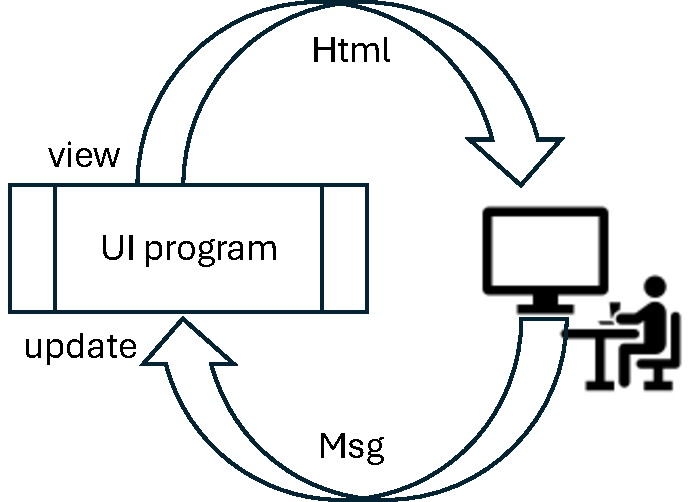
\includegraphics[width=0.6\columnwidth]{model-view-update}
  \caption{The Model-View-Update pattern}
  \Description{A diagram illustrating the flow in the
    Model-View-Update pattern: On the left is the program, on the
    right the user at the computer.  An arrow labeled ``view'' goes
    from the program to the computer, also labeled to carry HTML.
    Another arrow labeled ``update'' goes in the opposite direction,
    labeled to carry \texttt{Msg}.}
  \label{fig:mvu}
  \Description{The diagram shows a process box on the left
    representing the UI program, and a screen with a person sitting in
    front on the right.  The UI program box has an arrow coming out at
    the top, in a place labelled ``view'', with the arrow itself
    labelled ``Html'', and pointing to the screen.  The UI program box
    also has an arrow coming in, in a place labelled ``update'', with
    the arrow itself labelled ``Msg''.}
\end{figure}
%
Figure~\ref{fig:mvu} illustrates the pattern.
The \texttt{view} function constructs the UI, represented as a HTML
tree.  Each interactive UI widget carries a message of the
\texttt{Msg} type (also defined by the UI program) that is generated
when the user interacts with the widget.  The Elm toolkit then passes
this message to the \texttt{update} function that generates a new
model, which again gets fed into \texttt{view} and so on.

The \texttt{Cmd} type allows triggering impure actions outside of user
interactions.  In particular, a program performs network requests by
issuing commands, which get executed asynchronously and result in
incoming messages, thus ameliorating issues with JavaScript's
inherent event loop.

View-Model-Update is simple and easy to
learn, and does not require the developer to know higher-level
abstractions like signals, stream transformers or monads.  It also
avoids the circular dependency between view and model.

Model-View-Update is quite similar to Racket's
Universe teachpack: The view is re-constructed after every user
interaction, and it uses a single, monolithic value for the model
state.  The possible messages belong to a
single central type.
Consequently, Elm also inherits the Universe teachpack's architectural
trade-offs: It solves the \hyperlink{challenge:update}{\textit{Update}} challenge from Section~\ref{sec:challenges},
but has no notion of an
independent, composable ``UI component'' and thus faces the
\hyperlink{challenge:modularity}{\textit{Modularity}} challenge.

Shortly after Elm's initial release, Facebook released their web UI
toolkit \textit{React}, which was also based on a variation of the
Model-View-Update paradigm.
React's \texttt{render} function corresponds to Elm's \texttt{view}:
It transforms the model state into a HTML tree.  Unlike Elm,
React has a notion of a UI component---a sub-view with its
own associated state.

Where Elm gives the UI program complete freedom in the choice of
\texttt{Model} type, React differentiates two kinds of state:
Immutable \textit{properties} flow downward in the sub-view
tree---the property of a sub-view needs to be extractable purely from the
property of its parent.  Properties face the
\hyperlink{challenge:modularity}{\textit{Modularity}} challenge.
Each component also has its own associated mutable \textit{state},
which needs to be a JavaScript hash map.

Thus, React's model of reactivity is different from Elm's: The UI
program attaches imperative callbacks to UI components, and these
callbacks can either mutate the component state or cause the
properties to be replaced.  Conceptually, React ignores the difference
between these two methods and re-renders the entire UI on each
interaction, just like Elm.

Both React and Elm leave solving the
\hyperlink{challenge:modularity}{\textit{Modularity}} challenge to the
developers, and the communities of both have produced patterns to
alleviate the problem.

% FIXME: maybe notes on the implementation

Elm and React and the Model-View-Update pattern represented an
erstwhile peak in the evolution of functional APIs, intellectually
hailing from Fudgets and Fruit.  Consequently, we take
Model-View-Update as the starting point for the further discussion.

\section{UI Toolkits Elsewhere}
\label{sec:ui-toolkits-elsewhere}

Evolution did not just happen in functional approaches to UI
programming.  Object-oriented UI toolkits have also evolved,
specifically those for web applications.  Modern OO toolkits like
Angular, Svelte, and Vue.js have also attempted to solve the \hyperlink{challenge:update}{\textit{Update}} challenge
from Section~\ref{sec:challenges} using a common approach (also
available with React).

These toolkits rely on the same underlying architecture as the
original MVC pattern and require the program to construct the UI
initially and update specific parts of the UI corresponding to
specific changes in the model.  This way, they avoid the overhead of
Model-View-Update from (conceptually) re-constructing the UI on every
change.

However, instead of requiring the programmer to implement the update
logic manually, these toolkits feature a pre-processor 
that generates the update code automatically from the construction code.
This convenience comes at a price, as these toolkits require
the code changing the state to be exposed to the UI toolkit, and for
that code to use conventions recognizable to the pre-processor.  This
means that the model cannot be implemented independently of the UI
toolkit, and is thus coupled to the view---effectively giving up the
Model/View separation, the central tenet of MVC.

\section{Functional Modularity Challenges}
\label{sec:modularity-challenges}

Taking Elm's and React's Model-View-Update pattern as a starting
point, we summarize the architectural tradeoffs listed in
Section~\ref{sec:challenges}:
%
\begin{itemize}
\item Model-View-Update solves the \hyperlink{challenge:update}{\textit{Update}} challenge: A single function
  describes view construction, no separate logic for view update is
  needed.
\item The \hyperlink{challenge:modularity}{\textit{Modularity}} challenge---implementing modular sub-views---remains:
  A functional Elm/React application manages its model
  state as a single mutable reference at the top level, with
  everything below managed functionally.
\item Model-View-Update also solves the \hyperlink{challenge:circularity}{\textit{Circularity}} challenge, as the cyclic call
  chain is broken by the succession of models and updates
  presented to the UI toolkit.
\end{itemize}
%
Solving the \hyperlink{challenge:modularity}{\textit{Modularity}} challenge in the context of functional programming
means establishing a notion of ``UI
component'' without resorting to imperative state updates.  A solution
approach needs to address the facets described in this section: Updating
the model state in a modular fashion, dealing with UI-local state, and
breaking up global dispatch.

We illustrate these facets using a simple example: an
application that manages phone-book entries with name and phone
number.  The application manages the phonebook in a functional
manner, as a functional list of immutable entry records.  Its UI
contains a sub-view component that allows viewing and editing a single
name within a text field, along with a ``Submit'' button for actually
changing the phonebook.

% FIXME: maybe a figure

\subsection{Global Model State Update}

When the user changes the name, this is a local change from the point
of view of the UI component, but 
the application must update its global phonebook reference.  Thus,
updating the state is not the job of the name UI component
but of all the components above it in the hierarchy that need to
re-construct the state with the one changed name, and finally change
the global reference at the top.

\subsection{UI-Local State}

The model-state update happens when the user clicks the ``Submit''
button.  However, the UI has to manage the contents of the text field
as the user types in the new name one letter at a time.  This
intermediate state is of no interest to the model, hence it is
``UI-local'' and not an aspect
of the model.  Thus, the UI toolkit should enable separating the model state
from the UI-local state.

Note that the distinction between model state and UI-local state
depends on context and judgement: The name UI component itself has two
sub-components, a text field and the submit button.  The text field's
model will usually be the visible text.  However, embedded within the
name component, the text field's model state becomes the name
component's UI-local state.

\subsection{Global Dispatch}

In Elm, the UI program communicates requests to change the model state
(as well as other side effects) via messages of type \texttt{Msg},
which the toolkit subsequently passes to the \texttt{update} function.
This \texttt{update} function is global, and thus unmodular.  Making
the global dispatch modular requires associating it with an individual
UI component rather than the program as a whole.

However, a UI component is often not able to handle the messages
generated by user interaction with its view.  Consider again the name UI
component: The name should probably not be empty, and thus the
``Submit'' should be deactivated as long as the text field is empty.
Thus, the text-field component must pass a message upwards to its
enclosing name component, informing it of the state change.
Correspondingly, the enclosing component must be able to handle the
message coming up from its sub-component.

Furthermore, the type of the message produced by the sub-component
must match the type expected by the enclosing component.  This is not
necessarily the case when the two are developed separately: For this
case, the UI toolkit must offer a mechanism to transform the message
along the way from its producer to its handler.

\section{From Model-View-Update to Reacl}
\label{sec:reacl}

As a response to challenges described in the previous section, we
started in 2014 to work on our own UI toolkit for ClojureScript,
\textit{Reacl}~\cite{Reacl}.  Reacl is similar to Halogen, a UI
toolkit for PureScript~\cite{Halogen}, even though both were developed
independently.
This section describes how Reacl tackles
the modularity challenges, using the phonebook example.  Reacl evolved
significantly over its lifetime, eventually leading to its successor
reacl-c described in Section~\ref{sec:reacl-c}.  We describe Reacl version 2
from about 2019.

The phonebook example starts with a namespace declaration that imports
both Reacl and the record library from \textit{Active
  Data}~\cite{ActiveData}, a library for making data modeling
explicit:
%
\begin{verbatim}
(ns phonebook
  (:require
    [reacl2.core :as reacl :include-macros true]
    [reacl2.dom :as dom :include-macros true]
    [active.data.record :as record
      :include-macros true
      :refer-macros (def-record)]
    [active.data.realm :as realm]))
\end{verbatim}
%
We use Active Data to define a record type for an entry in the
phonebook, the central aspect of the model:
%
\begin{verbatim}
(def-record entry
  [entry-name :- realm/string
   entry-phone-number :- realm/string])
\end{verbatim}
%
In this declaration, \texttt{entry} is both the record type and
constructor, \texttt{entry-name},
\texttt{entry-phone-number} each double as field name and
getter/selector.  The \texttt{realm/} annotations declare the run-time
types of the fields of the record.

We now construct a UI for editing the name of an entry.  To that end,
we start with a reusable component for an editable text field.  This
is implemented via a \textit{class} in Reacl that defines how the
text-field components are rendered and behave:
%
\begin{verbatim}
(def-record change-text
  [change-text-text :- realm/string])

(reacl/defclass text-field this text []
  render
  (dom/input {:onchange 
              (fn [e]
                (reacl/send-message!
                 this
                 (change-text
                   change-text-text
                   (.. e -target -value))))
              :value text})
  handle-message
  (fn [msg]
    (cond
      (record/is-a? change-text msg)
      (reacl/return
        :app-state (change-text-text msg)))))
\end{verbatim}
%
In this declaration, \texttt{this} is the name that the code can use
to refer to the current component (similar to \texttt{this} in Java),
and \texttt{text} is the \textit{app state} of the component---its
model.

Two clauses follow, the first of which is \texttt{render}, which
generates the view from the app state \texttt{text}.  This is
straightforward HTML with a callback attached that fires whenever the
user changes the text.  The callback sends a
message to the component that describes the user's intention,
in this case to change the text in the form of a \texttt{change-text}
record.

Components can send messages to arbitrary other components, but it is
typical to send them ``to themselves,'' as is shown here.  The
\texttt{handle-message} clause defines how a component reacts to a
message it receives.  In this case, the only possible message is a
\texttt{change-text} record, but often components allow for more than
one kind of interaction, which is why there is a \texttt{cond} here that
identifies the \texttt{change-text} record.  The function then calls
\texttt{reacl/return}, which tells Reacl what
to do---in this case replace the app state of the component with the
text from the message, performing an update as in the
Model-View-Update pattern.\footnote{Since the development of Reacl,
  React has adopted a similar mechanism to \texttt{handle-message}
  called \textit{reducers}.}

In principle, the callback attached to the text field could itself
perform the update---first creating and then dispatching on a message
is more work.  However, this separation of concerns makes the
\texttt{handle-message} function testable, even outside of the running
UI application.  (The \texttt{render} function is also testable by
inspecting the returned HTML, but this comes with caveats described in
Section~\ref{sec:vague-semantics}.)

Next, we create a UI component for actually editing a name from a
phonebook.  The idea is that the phonebook will only be changed when
the user clicks on a \texttt{Submit} button.  Consequently, the app
state of the name component will only
change when \texttt{Submit} is pressed.  However, the component still
needs to keep track of current content of the text field.  To that
end, it keeps a \textit{local state}, which is not reflected in the
model state.  The class starts like this:
%
\begin{verbatim}
(reacl/defclass text-editor
  this text []
  local-state [current-text text]
\end{verbatim}
%
Here, \texttt{text} is the app state of the component.  The local
state is called \texttt{current-name} and its initial value upon
creation of the component is \texttt{text}.  Here is the
\texttt{render} clause, which creates an HTML form:
%
\begin{verbatim}
render
(dom/form
 {:onsubmit
   (fn [e] (.preventDefault e)
           (reacl/send-message! this (submit)))}
 (dom/div (text-field
           (reacl/opt
             :reaction
             (reacl/reaction
               this
               (fn [text]
                 (change-text
                   change-text-text text))))
           current-text)
          (dom/button "Submit")))
\end{verbatim}
%
This calls \texttt{text-field} to create a text-field component,
passing it a \textit{reaction} and \texttt{current-text} as its app
state.  (This shows that one component's app state can be another
component's local state.)  The reaction defines how the
\texttt{text-editor} component reacts to changes in the
\texttt{text-field} component's app state (passed in as \texttt{text}
to the function), typically by sending a message.  Here, the reaction
sends a \texttt{change-text} message (re-used from
\texttt{text-field)} to \texttt{this}.

The form callback, which gets called when the user clicks
\texttt{Submit}, sends a singleton \texttt{submit} message as per this
record declaration:
%
\begin{verbatim}
(def-record submit [])
\end{verbatim}
%
(The \texttt{.preventDefault} DOM call is just a technical necessity.)

Finally, the \texttt{handle-message} function dispatches on the two
messages, updating the local state for \texttt{change-name} and the
app state for \texttt{submit}:
%
\begin{verbatim}
handle-message
(fn [msg]
  (cond
    (record/is-a? change-name msg)
    (reacl/return
      :local-state (change-name-text msg))
    (record/is-a? submit msg)
    (reacl/return :app-state current-name))))
\end{verbatim}
%
This example shows how Reacl deals with the three challenges described
in Section~\ref{sec:modularity-challenges}:
%
\begin{description}
\item[Global Model State Update] A \texttt{handle-message} function
  only describes how to update its own model/app state, with no
  knowledge of and therefore no coupling to the global state of the
  application.
\item[UI-Local State] The \texttt{local-state} mechanism keeps local
  state out of the model.
\item[Global Dispatch] The \texttt{handle-message} function is per
  component class, no global dispatch is necessary.
\end{description}
%
It should be noted that Reacl also has a mechanism not described here
for side effects external to the UI component 
such as network
communication.  In order to make the core of the UI application pure,
it creates an \textit{action}, which is similar to a message with the
difference that it does not specify a receiver but gets propagated
upwards in the tree formed by the components until a component either
handles it or transforms it into an action understood further up.
This achieves modularity for actions in a way similar to reactions.

\section{Inherently Vague Semantics}
\label{sec:vague-semantics}

User interface construction remains a struggle. In addition to
the challenges described above, UI programming---and testing---is
difficult for reasons beyond the grasp of UI
tools.

Model-View-Update should make UI tests easy: Run the
\texttt{view }function for a sample \texttt{state} of
your domain logic and compare the resulting graphical display
\texttt{(view state)} to your desired version. Even forgetting about
the dynamic nature of UIs for a moment, this approach rarely results
in good tests. Take this temperature display in pseudocode:
%
\begin{verbatim}
(defn view [temp]
  (dom/div
    {:style (if (too-hot? temp)
              "background: red;" "")}
    (temperature->string temp))
(assert-equal (view 22) (dom/div "22")
(assert-equal (view 183)
  (dom/div {:style "background: red;"} "183"))
\end{verbatim}
%
This trivial test is problematic if we want to emphasize
not with a red background but a border.  Our test
demands that the background be red. To make the change,
we have to adapt both our implementation \textit{and} our
test.

A good
test checks whether an implementation satisfies a given specification.
Howeber, the specification of a
UI components is hard to separate from its implementation.
In this case, we want to ensure ``emphasis'', which 
is hard to formalize. Moreover, users' habits and expectations
change: An emphasis today might have been overlooked ten years ago. Additionally,
context is important. A graphical representation that is
emphatic when surrounded by white space may appears too timid
surrounded by loud advertisements.

Lehman's SPE classification~\cite{SPE} distinguishes programs
depending on how well specified and specifiable they are.
\textit{S} is for ``programs whose function is formally defined by and
derivable from a specification'', \textit{P} is for programs that have
a formal specification, but ``the acceptability of a solution is
determined by the environment in which it is embedded'', and
\textit{E} is for ``programs that mechanize a human or societal
activity''. Classes \textit{P} and \textit{E} are further aggregated
to form class \textit{A}---programs ``that represent a computer
application in the real world''. The distinction between \textit{S}
and \textit{A} programs aligns with our distinction between software
aspects that have a precise formal semantics and vague aspects like
emphasis. \textit{S} programs are amenable to automated tests
or even formal verification. \textit{A} programs on the other hand require manual tests to
verify their correctness.

While most UI software falls into the \textit{A} class \textit{in its
  entirety}, large software is made from smaller parts, which in turn
can be classified as either \textit{S} or \textit{A}. In the
temperature display example above, 
emphasis is the problematic aspect in terms of precise formal
specification---an \textit{A} aspect. In contrast, the function
\texttt{tooHot} solely operates in terms of the core domain
logic, and is independent of its context or any human habits
or practices---it belongs to class \textit{S}.

This S/A separation also applies to Reacl's separation between a UI
widget's event handler, the representation of the user's intention,
and its dispatch in the \texttt{handle-message} function.  All fall
squarely within class A, which makes the separation less valuable than
it might seem from a purely architectural perspective.

In order to bring down the costs of tests, we have to strive for
a separation of \textit{S} software parts from
\textit{A} software parts, and thus we want to write as little
UI code as possible. In the remainder of this work we propose a
discipline that supports this goal: we introduce reacl-c, a UI
combinator library that is optimized for reusability and we make a
case for the \textit{functional view model}, a UI programming
pattern.

\section{From Reacl to reacl-c}
\label{sec:reacl-c}

Reacl allows for many different styles of component
composition, which makes it hard to write widely applicable reusable
abstractions. Over the years, patterns for
Reacl components emerged, eventually leading to the creation of the \textit{reacl-c}
library~\cite{reacl-c}.
The differences between Reacl and reacl-c focus on the relationship
between components, and at what time the relationship is
defined.  Consider the call to \texttt{text-field} in the
phonebook example:
The reaction is part of the \texttt{text-editor} \emph{class}, and
thus effectively has to be the same for all components of that
class---it's decided statically.

A developer might want to defer the decision on the reaction until run time,
maybe because they want to use a
component combinator that has to operate on state as well.
In that case, they have
to write a function that takes the \texttt{reacl/opt} value and
\texttt{current-name} as arguments and build a combinator
that works on these component constructor functions (instead of
working on components), which is awkwardly indirect.
To that end, reacl-c does away with the
separation between classes and their components.

Another pattern that emerged from experience with Reacl
is the relationship between parent
and child, which is often best described by a lens~\cite{Lenses}:
A child component is often responsible for part of its parent's
state. That means that the data flow from parent to child works like
the \texttt{GET} operation of a suitable lens and the data flow from
child to parent corresponds to the \texttt{PUTBACK} operation.

\subsection{User-Interface Combinators}

reacl-c inherits the Model-View-Update paradigm from Reacl.  State is kept local to each item. The relationship between
the states of two different items is mostly expressed with lenses.  reacl-c's small
set of flexible combinators allows developers to express abstractions
that increase reuse and help sharply delineate the distinction of S
and A code.

The unit of
composition in reacl-c is called \textit{item}. All reacl-c items have
a notion of state, items may have a visual appearance, items may issue
actions and messages, and items may perform controlled effects.  For
this overview it suffices to focus on (DOM) visuals and state.
An item has the (imaginary) type \texttt{Item
  state}, where \texttt{state} is the type of the item's state.

Strings are primitive, state-agnostic items that simply display as
themselves:
%
\begin{verbatim}
"Hello" : forall s. Item s
\end{verbatim}
%
The \texttt{div} DOM combinator combines multiple items into
one and allow adding additional styling. Given two items \texttt{i}
and \texttt{j} of type \texttt{Item s}, the new item
%
\begin{verbatim}
(div {:style {:border "1px solid blue"}}
     i j) : Item s
\end{verbatim}
%
displays \texttt{i} and \texttt{j}
side-by-side (or on top of each other, depending on circumstances
outside of the scope of this discussion) and draws a blue
border around them. Optionally, these DOM combinators take special
arguments that allow users to update state. The item
%
\begin{verbatim}
(button
 {:onClick (fn [x] (+ x 1))} "Inc") : Item Int
\end{verbatim}
%
displays a button with the label ``Inc'' that increments its state
when the user clicks. The handler function argument takes the current state as its
first argument and returns a new state value for the next logical UI
cycle.

\texttt{focus} is an item combinator that takes an
item that operates on state of type \texttt{s} and a lens between
types \texttt{s} and \texttt{t} and returns a new item that operates
on type \texttt{t}.  Given the increment button above as
\texttt{incButton}, we can build a GUI for a tuple of two integers by
combining \texttt{focus} and \texttt{div}:
%
\begin{verbatim}
(div
 (focus lens/first incBut)
 (focus lens/second incBut)) : Item (Int, Int)
\end{verbatim}
%
All items above only update
state but never display it. That's where the \texttt{dynamic} item
constructor comes into play:
%
\begin{verbatim}
dynamic : forall s.(s -> Item s) -> Item s
\end{verbatim}
%
This takes a
function that gets the current state of type \texttt{s} 
and produces an item with that same state type. We can use
\texttt{dynamic} to build an increment button that displays the
current value as its label:
%
\begin{verbatim}
(c/dynamic
 (fn [i]
  (button {:onClick (fn [x] (+ x 1)} (str i)))))
\end{verbatim}
%
The item combinator
%
\begin{verbatim}
isolate-state : forall s t.t -> Item t -> Item s
\end{verbatim}
%
takes an initial value of type \texttt{t} and an item of
type \texttt{Item t} and ``runs'' the item with the given initial
state value. The resulting item can be used in any state context. This
detaches an item's state from its surrounding
state.
A less drastic combinator is
%
\begin{verbatim}
local-state : forall s t.t -> Item (s, t) -> Item s
\end{verbatim}
%
which takes an initial value of type \texttt{t} and an item that
operates on state of type \texttt{(s, t)}. The result is an item that
operates on state of type \texttt{s}. From the perspective
of the parent item, \texttt{local-state} introduces the right part of
the state tuple to form the child's state. When viewed from the
perspective of the child item, \texttt{local-state} hides the right
part of the state tuple from the parent.

These combinators (along with a handful of others) enable programming
techniques from pure functional programming to be carried over to GUI
construction.

\subsection{Phonebooks Redux}

To further illustrate reacl-c, we re-use the phonebook domain model 
from section~\ref{sec:reacl-c}.  We import the reacl-c namespaces along with
\texttt{active.data} and \texttt{active.clojure}.
%
\begin{verbatim}
(ns phonebook
  (:require
    [reacl-c.core :as c :include-macros true]
    [reacl-c.dom :as dom :include-macros true]
    [reacl-c.main :as cmain]
    [active.clojure.lens :as lens]
    [active.data.record :refer-macros [def-record]]
    [active.data.realm :as realm]))
\end{verbatim}
%
For our phonebook GUI we need a text-field, which we can build
with a combination of \texttt{c/dynamic} and \texttt{dom/input}.
%
\begin{verbatim}
(def text-field
  (c/dynamic
   (fn [text]
    (dom/input
     {:value text
      :onChange (fn [old-text event]
                  (.-value (.-target event)))}))))
\end{verbatim}
%
As shown above the \texttt{:onChange} handler describes how to update
the current state.  Here we see how reacl-c integrates with the native
DOM bedrock of the browser: The \texttt{:onChange} handler takes a
native DOM event object as an optional second
parameter that contains the desired result text.

We can build a text editor with a Submit button, similar to the Reacl
version above with the help of \texttt{local-state}. Here we can reuse
\texttt{text-field} unmodified.
%
\begin{verbatim}
(def text-editor
  (c/dynamic
   (fn [text]
     (c/local-state
      text
      (dom/form
       {:onSubmit
         (fn [[outer-text current-text] event]
           (.preventDefault event)
           [current-text current-text])}
       (c/focus lens/second text-field)
       (dom/button {:type "submit"} "Submit"))))))
\end{verbatim}
%
The \texttt{local-state} function pairs local state \texttt{current-text}
with the item's state, called \texttt{outer-text} in the submit
callback.  (Thus, differently from Reacl, the local state becomes part
of the state rather than being bound to a separate variable.)  The
call to \texttt{focus} that embeds \texttt{text-field} focusses the
\texttt{text-field} component on that local state.
%
\begin{center}
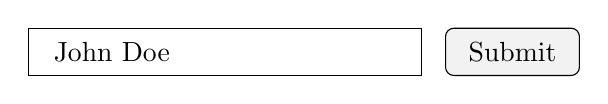
\begin{tikzpicture}

% Text field
\draw (0,0) rectangle (5,0.6);
\node[anchor=west] at (0.2,0.3) {John Doe};

% Button
\draw[fill=gray!10,rounded corners=3pt] (5.3,0) rectangle (7,0.6);
\node at (6.15,0.3) {Submit};

\end{tikzpicture}
\end{center}
%
Many relationships between different parts of GUI applications can be
expressed as lenses, so the \texttt{focus} combinator makes for 
powerful glue.  (Record field names defined by \texttt{def-record} from
\texttt{active.data.record} are also lenses.) The following
example shows a small UI that manages a single entry in our phonebook
application.
%
\begin{verbatim}
(def entry-item
  (dom/div "Name:" (c/focus entry-name text-editor)
           "Tel:" (c/focus entry-phone-number
                           text-editor)))
\end{verbatim}
%
\begin{center}
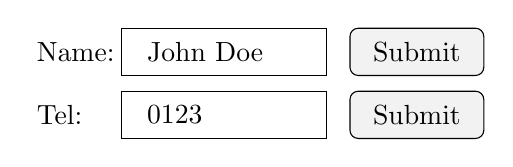
\begin{tikzpicture}

% Text field
\node[anchor=west] at (0.2,0.3) {Name:};
\draw (1.4,0) rectangle (4.0,0.6);
\node[anchor=west] at (1.6,0.3) {John Doe};

% Button
\draw[fill=gray!10,rounded corners=3pt] (4.3,0) rectangle (6,0.6);
\node at (5.15,0.3) {Submit};

\begin{scope}[yshift=-0.8cm]
% Text field
\node[anchor=west] at (0.2,0.3) {Tel:};
\draw (1.4,0) rectangle (4.0,0.6);
\node[anchor=west] at (1.6,0.3) {0123};

% Button
\draw[fill=gray!10,rounded corners=3pt] (4.3,0) rectangle (6,0.6);
\node at (5.15,0.3) {Submit};
\end{scope}

\end{tikzpicture}
\end{center}
%
We can evolve this
single phonebook entry to an item that manages an
entire phonebook (a sequence of entries) by using \texttt{focus}
with a lens:
%
\begin{verbatim}
(def phonebook
  (c/dynamic
   (fn [entries]
     (apply
      dom/div
      (map (fn [idx]
             (c/focus (lens/at-index idx)
                      entry-item))
           (range (count entries)))))))
\end{verbatim}
%
Here we map over the indices of the entries in the phonebook and use
\texttt{(c/focus (lens/at-index idx) ...)} to focus on the \texttt{entry}
item for each phonebook entry.
%
This pattern is very common when
dealing with lists, and we can
distill it into a custom combinator:
%
\begin{verbatim}
(defn map-item [child-item]
  (c/dynamic
   (fn [xs]
     (apply
      dom/div
      (map (fn [idx]
             (c/focus (lens/at-index idx)
                      child-item))
           (range (count xs)))))))
(def phonebook-2 (map-item entry))
\end{verbatim}
%
In contrast to Reacl components, items such as \texttt{child-item} are
not wired to any other UI widgets, so the \texttt{map-item} combinator
can use \texttt{focus} to establish a connection between its state and
\texttt{child-item}'s state.
Here, we add
a button that inserts a new entry into the
phonebook, which works with the entire phonebook state.
%
\begin{verbatim}
(def empty-entry
  (entry entry-name "" entry-phone-number ""))
(def phonebook-with-add-button
  (dom/div
   phonebook-2
   (dom/button
    {:onClick
     (fn [phonebook _] (conj phonebook empty-entry))}
    "Add new")))
\end{verbatim}
%
\begin{center}
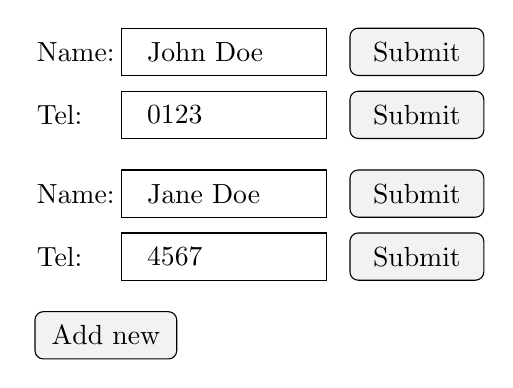
\begin{tikzpicture}

% Text field
\node[anchor=west] at (0.2,0.3) {Name:};
\draw (1.4,0) rectangle (4.0,0.6);
\node[anchor=west] at (1.6,0.3) {John Doe};

% Button
\draw[fill=gray!10,rounded corners=3pt] (4.3,0) rectangle (6,0.6);
\node at (5.15,0.3) {Submit};

\begin{scope}[yshift=-0.8cm]
  % Text field
  \node[anchor=west] at (0.2,0.3) {Tel:};
  \draw (1.4,0) rectangle (4.0,0.6);
  \node[anchor=west] at (1.6,0.3) {0123};

  % Button
  \draw[fill=gray!10,rounded corners=3pt] (4.3,0) rectangle (6,0.6);
  \node at (5.15,0.3) {Submit};
\end{scope}

\begin{scope}[yshift=-1.8cm]
  % Text field
  \node[anchor=west] at (0.2,0.3) {Name:};
  \draw (1.4,0) rectangle (4.0,0.6);
  \node[anchor=west] at (1.6,0.3) {Jane Doe};

  % Button
  \draw[fill=gray!10,rounded corners=3pt] (4.3,0) rectangle (6,0.6);
  \node at (5.15,0.3) {Submit};

  \begin{scope}[yshift=-0.8cm]
    % Text field
    \node[anchor=west] at (0.2,0.3) {Tel:};
    \draw (1.4,0) rectangle (4.0,0.6);
    \node[anchor=west] at (1.6,0.3) {4567};

    % Button
    \draw[fill=gray!10,rounded corners=3pt] (4.3,0) rectangle (6,0.6);
    \node at (5.15,0.3) {Submit};
  \end{scope}
\end{scope}

\begin{scope}[yshift=-3.6cm]
    % Add new button
    \draw[fill=gray!10,rounded corners=3pt] (0.3,0) rectangle (2.1,0.6);
    \node at (1.2,0.3) {Add new};
\end{scope}

\end{tikzpicture}
\end{center}

\section{The View Model, Functionally}

In the phonebook application above, when a user clicks the ``Add
new'' button, the application inserts a new entry below the others. The user can
then click on the name input field and enter the new entry's name. The
newly inserted widget looks like any other list item, however. In
order to give the user explicit feedback as to what happened on
screen, we now want to highlight newly inserted entries. As we argued
in Section~\ref{sec:vague-semantics}, it is hard to formally specify what it means exactly for a UI
widget to be emphasized. We should still extract the notion of
emphasis into an isolated item combinator:
%
\begin{verbatim}
(defn emphasize [item]
  (dom/div {:style {:border "1px solid blue"}}
           item))
\end{verbatim}
%
So far the domain model and the state of our items have been the same. Now
we also have to keep track of which entry to \texttt{emphasize}. We
therefore separate our domain model from the model of our UI state. This
is a pattern well-known in the OO community
as ``Model-View-ViewModel'' (MVVM)~\cite{MVVM}.
Our view model includes a phonebook entry from the core domain model,
enriched with the information whether this particular entry should be
emphasized. A phonebook view model consists of a sequence of such
entries.
%
\begin{verbatim}
(def-record entry-vm
  [entry-vm-entry :- entry
   entry-vm-emphasized? :- realm/boolean])
\end{verbatim}
%
It probably doesn't make sense to have more than one \texttt{entry} with
\texttt{entry-vm-emphasized?} set to \texttt{true}. We provide a set of smart
constructors and accessors that keep the constraint satisfied. First,
we need an empty phonebook:
%
\begin{verbatim}
(def empty-phonebook [])
\end{verbatim}
%
In our minimal phonebook example the only way to build larger phone
books is to use an \texttt{add-new-entry} function:
%
\begin{verbatim}
(defn deemphasize [entry]
  (entry-vm-emphasized? entry false))
(defn add-new-entry [entries]
  (conj (mapv deemphasize entries)
        (entry-vm entry-vm-entry empty-entry
                  entry-vm-emphasized? true)))
\end{verbatim}
%
\texttt{add-new-entry} is a pure function with precise semantics and
thus a perfect candidate for testing.

These definitions constitute our view model. The corresponding
UI code is straightforward. The new entry item \texttt{entry-item-2}
handles emphasis conditionally and then delegates on to the
\texttt{entry-item} defined above.
%
\begin{verbatim}
(def entry-item-2
  (c/dynamic
   (fn [entry-vm]
     ((if (entry-vm-emphasized? entry-vm)
        emphasize identity)
      (c/focus entry-vm-entry entry-item)))))
(def phonebook-item-2 (map-item entry-item-2))
\end{verbatim}
%
The phonebook still needs an ``Add new'' button. This button
now simply calls \texttt{add-new-entry}:
%
\begin{verbatim}
(def phonebook-with-add-button-item-2
  (dom/div phonebook-item-2
           (dom/button {:onClick add-new-entry}
                       "Add new")))
\end{verbatim}
%
The view-model pattern enabled by reacl-c allows moving part of the UI
into S realm of the SPE classification.  This yields the important
architectural benefits of the Reacl model: no separate update code,
modular components, no circular callbacks.  Separating out the view
model further enables testability in the parts of the UI code where it
makes sense, and minimizes the amount of code where it does not.

\section{Conclusion}
\label{sec:conclusion}

UI programming and the architecture of UI program have evolved
significantly since the MVC pattern, but the basic tenets of
MVC are still in place.  Object-oriented and functional approaches
have had complementary trade-offs: Pure MVC featured good modularity
from the start, but has struggled with keeping the view current with
respect to the view.
Conversely, the functional Model-View-Update pattern in its pure form
solves the update problem but struggles with modularity.  We have
described the Reacl and reacl-c UI toolkits that address the
modularity issues with Model-View-Update, and shown how to enhance
Model-View-Update with functional view models to further modularize UI
programs.

\begin{acks}
  We thank David Frese, the principal designer of reacl-c, for
  assistance with the example code.  We also thank the reviewers for
  their helpful comments.
\end{acks}

%%
%% The next two lines define the bibliography style to be used, and
%% the bibliography file.
\bibliographystyle{ACM-Reference-Format}
\bibliography{funarch-ui}

\end{document}
\endinput
%%
% TODOs:
% - cite Conal


